% 双原子分子势能曲线

\subsection{双原子分子势能曲线}
\textbf{双原子分子势能曲线(Potential Energy Curves)}是认识和描述双原子分子、离子动力学最方便的工具之一,在研究双原子分子、离子的过程中被广泛地使用.
它的横坐标是原子间距,纵坐标是势能.一个典型的双原子分子势能曲线如图1\footnote{图片来自:Li,H,et al."Intensity dependence of the attosecond control of the dissociative ionization of D2." Journal of Physics B Atomic Molecular & Optical Physics 47.12(2014):124020}

\begin{figure}[ht]
\centering
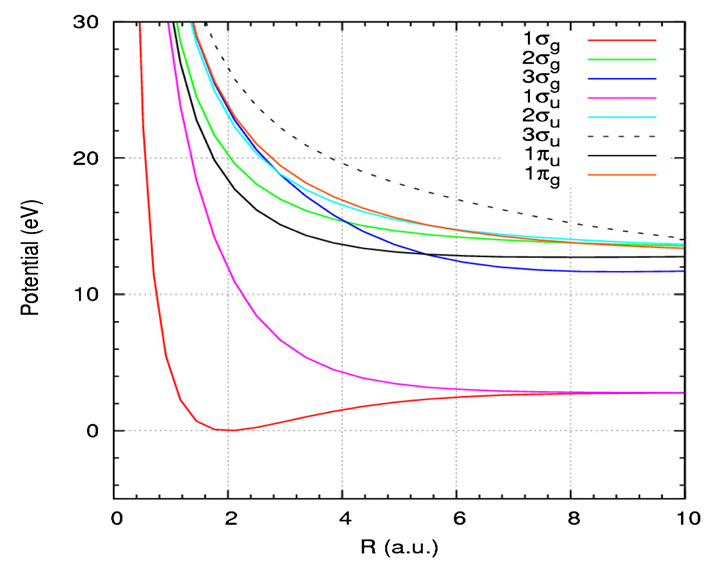
\includegraphics[width=10cm]{./figures/dpecs_1.png}
\caption{$D_2^+势能曲线图$} \label{dpecs_fig1}
\end{figure}
通常在双原子分子势能曲线图中,不同电子态的曲线会在势能曲线旁边标注.通过使用势能曲线,我们可以更好地认识和描述双原子分子的电离、解离等过程.

